\documentclass[12pt]{article}

\usepackage[margin=1in]{geometry}
\usepackage[british]{babel}
\usepackage[style=american]{csquotes}
\usepackage{orcidlink}
\usepackage{fontspec}
\setmainfont{Charis SIL} % compile with LuaLaTeX or XeLaTeX
\usepackage[final]{microtype}
\usepackage{marvosym}
\usepackage{enumitem}
\usepackage{hyperref}
\usepackage{tikz}
\usetikzlibrary{shapes,arrows,positioning,fit,backgrounds,calc}
\hypersetup{
    colorlinks=true,
    linkcolor=blue,
    citecolor=blue,
    pdfauthor={Brett Reynolds},
    pdftitle={Naturalizing Typological Kinds: Comparanda, Mechanisms, and Measurement}
}

\usepackage{amssymb,amsmath}
\usepackage{graphicx}
\usepackage{langsci-gb4e}

\usepackage{array,booktabs} % booktabs optional but recommended
\newcolumntype{L}[1]{>{\raggedright\arraybackslash}p{#1}}


\usepackage[style=apa,backend=biber]{biblatex}
\DeclareLanguageMapping{british}{british-apa}
\addbibresource{references.bib}

% House style macros
\newcommand{\term}[1]{\textit{#1}}

% Subscript notation macros for comparanda
% \Cross from amssymb is used directly (proper cross symbol)
\newcommand{\Eng}{Eng}
\newcommand{\Jpn}{Jpn}
\newcommand{\Spn}{Spn}
\newcommand{\Tha}{Tha}
\newcommand{\Rus}{Rus}
\newcommand{\Lat}{Lat}
\newcommand{\Hbr}{Hbr}
\newcommand{\Lgr}{$L$}  % Generic language variable

\title{Naturalizing Typological Kinds:\\Comparanda, Mechanisms, and Measurement}
\author{Brett Reynolds \orcidlink{0000-0003-0073-7195}\thanks{I used ChatGPT 5, Claude Sonnet 4.5, Gemini Pro 2.5, and Kimi 2 extensively in drafting and revising the paper. I reviewed, edited, and approved all the material and take full responsibility for the final text and conclusions. \href{mailto:brett.reynolds@humber.ca}{brett.reynolds@humber.ca}}\\Humber Polytechnic \& University of Toronto}
\date{\today}


\begin{document}
\maketitle


\begin{abstract}
Why do typological universals keep dissolving? Because we measure the wrong things. We count articles and call it definiteness. We track nominative case and call it subjecthood. We confuse what we compare with how languages realize it, and the universals evaporate. When English \textsc{noun}\textsubscript{Eng} or Hebrew \textsc{subject}\textsubscript{Heb} is projected directly onto a purportedly universal \textsc{noun}\textsubscript{\Cross}, measurement error and spurious asymmetries accumulate.

I propose a homeostatic framework that keeps the levels apart and makes the explanatory work accountable. First, a three-tier \emph{comparanda--realization} mapping separates cross-linguistic functions, semantic targets, discourse roles, and categories from their language-specific realizations. Second, a \emph{syntax--semantics firewall} separates diagnostic evidence from morphosyntactic form, ensuring that comparative concepts travel without dragging language-particular packaging. Third, some comparanda earn promotion to \emph{naturalized comparative concepts} when convergent cognitive, discourse, diachronic, or community mechanisms maintain their property clusters; others are tagged with explicit failure modes.

The framework issues risk-bearing predictions about trade-offs, regeneration pathways, and latent-variable diagnostics (e.g., \emph{nominality}) and is formalized in an auditable specification (\texttt{src/typology.py}). By demanding mechanisms as well as mappings, the account preserves the empirical ambition of typology while avoiding the universalist overreach that has long haunted the field.
\end{abstract}

\section{Orientation}\label{sec:orientation}
Two requirements conflict: cross-linguistic comparison needs predicates that travel across grammars, while grammatical analysis needs kinds that are grammar-specific. From this tension, typology accumulates measurement error and fragile generalizations.

I adopt a terminological discipline following \textcite{HuddlestonPullum2002}: \emph{function} (unqualified) denotes syntactic functions only; \emph{target} denotes semantic targets; \emph{role} denotes discourse/pragmatic roles; \emph{category} denotes syntactic categories. Subscripts distinguish comparative cross-linguistic concepts (\textsc{term}\textsubscript{\Cross}) from language-specific realizations (\textsc{term}\textsubscript{Eng}, \textsc{term}\textsubscript{Jpn}) and general language-internal references (\textsc{term}\textsubscript{$L$}) where no particular language is in focus.

Following \textcite{Haspelmath2010}, I treat cross-language targets as \emph{comparative concepts}~-- analyst-constructed categories that allow comparison without assuming the categories exist in individual grammars. Building on \textcite{Croft2001,HuddlestonPullum2002}, I analyse language-internal lexical categories as homeostatic property cluster (HPC) kinds~-- categories that persist because mechanisms maintain clustered properties, not because they have essential defining features \parencite{Boyd1991Enthusiasm,Boyd1999Homeostasis,Khalidi2013}. I call these cross-linguistic targets \emph{comparanda}~-- the phenomena we compare across languages, distinct from language-specific realizations.

The foundation: clear descriptions of language-internal syntactic categories and functions~-- English's noun, Japanese's relative clause, Hebrew's subject~-- with their full morphosyntactic property clusters. Cross-linguistic comparison then requires apparatus that permits asking whether English's noun and Japanese's noun realize similar patterns, without presupposing that English's cluster defines the universal or that cross-linguistic prototypes have to mirror any particular realization. Section~\ref{sec:failures} details how systematic conflation errors block this goal.


Table~\ref{tab:levels} presents the three-level ontology that separates what we compare across languages from what exists in particular grammars.

\begin{table}[ht]
  \centering
  \caption{Three-level ontology for comparative concepts and realizations}\label{tab:levels}
  \begin{tabular}{p{3cm}p{6.2cm}p{5.5cm}}
    \toprule
    Level & Contents & Diagnostic focus \\
    \midrule
    Level-I: \hspace{1.5cm} cross-linguistic pressures & Semantic targets (\textsc{specificity}\textsubscript{\Cross}, \textsc{definiteness}\textsubscript{\Cross}, \textsc{mass/count}\textsubscript{\Cross}) and discourse roles (\textsc{topic}\textsubscript{\Cross}, \textsc{focus}\textsubscript{\Cross}, \textsc{vocative}\textsubscript{\Cross}) & Behavioural tests on interpretation, common ground management, and discourse continuity \\ \addlinespace[4pt]
Level-II: \hspace{1.5cm} cross-linguistic syntax & Functions (\textsc{subject}\textsubscript{\Cross}, \textsc{head}\textsubscript{\Cross}, \textsc{predicate}\textsubscript{\Cross}) and categories (\textsc{V}\textsubscript{\Cross}, \textsc{VP}\textsubscript{\Cross}, \textsc{clause}\textsubscript{\Cross}) & Portable morphosyntactic diagnostics (alignment, extraction, agreement control, slot privileges) \\ \addlinespace[4pt]
Level-III: language-internal syntax & Language-internal functions (\textsc{subject}\textsubscript{Eng}, \textsc{head}\textsubscript{Spn}, \textsc{predicate}\textsubscript{Tha}) and categories (\textsc{V}\textsubscript{Eng}, \textsc{VP}\textsubscript{Mndr}, \textsc{clause}\textsubscript{Hbr}) & Distributional, morphological, and prosodic evidence specific to $L$; mapped to Level~II with graded weights \\ \addlinespace[4pt]
    \bottomrule
  \end{tabular}
\end{table}

Multiple levels may converge in a single expression. In [\textit{the cat}] \textit{awoke}, the bracketed NP instantiates \textsc{topic}\textsubscript{\Cross} (Level~I) and \textsc{subject}\textsubscript{\Cross} (Level~II) via the language-internal function \textsc{subject}\textsubscript{Eng} (Level~III).

Levels~I and~III persist as homeostatic property-cluster kinds sustained by different mechanisms: cognitive–interactional pressures stabilize Level~I, while community-internal morphosyntax and diachrony sustain Level~III. Level-II comparanda, by contrast, are analyst-proposed comparative concepts. Some may earn \emph{naturalized} status (Section~\ref{subsec:naturalization-criteria}) and be treated (defeasibly) as kinds; others remain instrumental comparanda without ontological commitment.

Three additions operationalize this framework: an executable three-level \emph{comparanda--realization} schema (Section~\ref{sec:matrix}) separating what we compare (categories\textsubscript{\Cross}, functions\textsubscript{\Cross}, targets\textsubscript{\Cross}, roles\textsubscript{\Cross}) from what exists in particular languages (language-specific category realizations); an explicit \emph{syntax--semantics firewall protocol} (Section~\ref{sec:hygiene}) testing semantic targets independently of their morphological or syntactic expression; and a measurement-first approach (Sections~\ref{sec:naturalized} and \ref{sec:measurement}) promoting some comparative concepts to \emph{naturalized} status when they show consistent cross-linguistic stability with identifiable homeostatic mechanisms.\footnote{A parallel object-oriented specification of these structures is maintained in \texttt{src/typology.py} to keep the theoretical machinery auditable.}

The paper proceeds as follows. Section~\ref{sec:failures} diagnoses four recurrent conflation errors in current typological practice, showing how they manifest in published research. Section~\ref{sec:matrix} operationalizes the three-level mapping with formal apparatus (mapping functions, weight assignment, reliability scores). Section~\ref{sec:hygiene} extends the framework to semantic targets through a firewall protocol with operational diagnostics. Sections~\ref{sec:naturalized} and \ref{subsec:mechanisms} introduce naturalized comparative concepts and the homeostatic mechanisms that stabilize them, with a biological interlude (Section~\ref{sec:eyes}) illustrating character-identity mechanisms. Section~\ref{sec:measurement} develops measurement models using latent variables. Section~\ref{sec:predictions} derives five falsifiable predictions with declared thresholds. Section~\ref{sec:illustrations} applies the framework to three typological debates. Section~\ref{sec:threats} addresses objections about measurement feasibility, falsifiability, and circularity.

\section{Where typology goes wrong}\label{sec:failures}
Systematic errors in published typological research trace to a single source: conflating comparanda (categories\textsubscript{\Cross}, functions\textsubscript{\Cross}, targets\textsubscript{\Cross}, roles\textsubscript{\Cross}) with language-internal categories\textsubscript{$L$} and $L$-functions, or meanings with forms. The confusions run bidirectionally~-- language-internal categories project onto comparative functions and vice versa; property clusters of local realizations project onto comparative notions and vice versa~-- generating four recurrent obstacles.

\subsection{Four obstacles manifested}\label{subsec:failure-modes}

\emph{Dual-use terminology and category--function conflation} (obstacle a) arises when the same label is pressed into service for different ontological levels, encouraging analysts (or readers) to treat unlike phenomena as identical. A textbook example is \term{determiner}: it often names an NP-internal syntactic function and, at the same time, the lexical category realized in English by words like \textit{the}, \textit{this}, \textit{many}.  \textcite{Reynolds2025Definiteness} has recently pointed out that \textit{definite} is used as both a semantic term and for the exponent that prototypically realize definite semantics. \textit{Adverb}(\textit{ial}) commonly confounds adjuncts in general with a lexical category that commonly functions as adjuncts. \textit{Topic} is used multiply for categories (e.g., \textit{topic marker}), a discourse/pragmatic role, and prosodic/intonational patterns. Although many linguists and laypeople are aware of this polysemy and try to guard against it, confusion abounds. Maintaining strict terminological discipline is best practice, even if that means creating vulgar neologisms.

\emph{Cluster reduction} (obstacle b) collapses a syntactic category's rich morphosyntactic property profile~-- distributional privileges, paradigmatic contrasts, agreement patterns, extraction behaviour~-- into a few semantic or discourse-functional properties; treating nouns as \enquote{thing-words} or subjects as \enquote{agents} discards the morphosyntactic evidence that defines these categories within their grammars.

\emph{Template import} (obstacle c) projects one language's morphosyntactic profile onto cross-linguistic prototypes: defining \textsc{subject}\textsubscript{\Cross} by properties of a particular category profile (nominative NP controlling agreement) bakes English or Russian structure into the comparative concept, producing tautologies (nominative languages trivially \enquote{have subjects}) or spurious counterexamples (ergative systems \enquote{lack subjects}) \parencite{Dryer1997,EvansLevinson2009}.

\emph{False universalisation} (obstacle d) assumes that every language must realise cross-linguistic prototypes with similar formal properties, generating undergeneralisation (\enquote{no adjectives $ \Rightarrow$ no property modification}) or overprojection (\enquote{no determiners $\Rightarrow$ no definiteness}). Yet functions and targets persist where their prototypical categories are absent: the \textsc{modifier}\textsubscript{\Cross} function survives via relative clauses, property nouns, or participles where \textsc{adjective}\textsubscript{$L$} categories are absent \parencite{Dixon2010,Croft2001}; the \textsc{definiteness}\textsubscript{\Cross} target persists via demonstratives, possessive frames, or classifier complexes where \textsc{determinative}\textsubscript{$L$} categories are absent. A related error conflates semantic or discourse targets with morphosyntactic exponents: \textsc{definiteness}\textsubscript{\Cross} becomes synonymous with articles, \textsc{specificity}\textsubscript{\Cross} with accusative case, \textsc{agentivity}\textsubscript{\Cross} with subjecthood. Reported \enquote{universals} then track \emph{exponents} rather than \emph{targets}, misdiagnosing languages that lack the exponent as lacking the target.

\subsection{Concrete illustrations}\label{subsec:compressed}

\begin{exe}
\ex\label{ex:determiner-double-duty}
\textbf{Category–function conflation: \textsc{determiner} (function) vs.~\textsc{determinative} (category).}
\textcite{QuirkEtAl1972} use \emph{determiner} for both an NP-internal \emph{function} and a lexical \emph{category} (words like \textit{the}, \textit{many}, \textit{which}, \textit{each}). The conflation arises because the prototypical determinative\textsubscript{Eng} realizes the determiner\textsubscript{Eng} function, but determinatives\textsubscript{Eng} also function as modifiers\textsubscript{Eng} (e.g., \textit{the }[\textit{many}]\textit{ books that we have}) while phrases of other categories\textsubscript{Eng} may realize determiner\textsubscript{Eng} function (e.g., the genitive NP\textsubscript{Eng} in [\textit{June's}] \textit{shoe}).

The distinction between what something is (\textsc{determinative}\textsubscript{Eng} category) and how it relates to other constituents (\textsc{determiner}\textsubscript{Eng} function) disappears. Cross-linguistic projection generates confusion: does Japanese \enquote{have determiners}? Without specifying whether we're asking about a lexical category or a syntactic function, the question is unanswerable.

\ex\label{ex:definiteness-vs-articlehood}
\textbf{Cluster reduction: \textsc{definiteness}\textsubscript{\Cross} (semantic target) vs.\ article systems (morphosyntactic category).}
Large typological surveys proxy \textsc{definiteness}\textsubscript{\Cross} by article presence: WALS 37A and APiCS chapter~28 code languages as \enquote{having definiteness} only if they grammaticalize dedicated definite articles \parencite{Dryer2013WALSDefArt,APiCS2013DefArticles}. Some analyses treat articleless systems as lacking presuppositional definiteness altogether \parencite{SimikDemian2020}. But  \textsc{definiteness}\textsubscript{\Cross}~-- identifiability via anaphoric uptake, uniqueness inferences, familiarity presuppositions~-- is a semantic target maintained by discourse-pragmatic mechanisms (common ground management, bridging, topic continuity), while article systems are morphosyntactic categories maintained by grammaticalization, acquisition, and community transmission. Though grammaticalization conventionalizes their pairing, systematic dissociation nevertheless occurs \parencite{Reynolds2025Definiteness}. Articles\textsubscript{Eng} prototypically signal \textsc{definiteness}\textsubscript{\Cross} in familiar European languages, but this correlation is a local fact, not a definitional requirement.

Cross-linguistic projection generates undergeneralization: languages without articles are misdiagnosed as lacking \textsc{definiteness}\textsubscript{\Cross} altogether, collapsing a rich semantic target into the presence of a single morphosyntactic exponent. Yet definiteness diagnostics~-- anaphora, uniqueness, anti-novelty contexts~-- still apply in articleless languages \parencite{Lyons1999,Matthewson2004}. Even English shows systematic divergences: weak definites (\textit{take the bus}) use the definite article without token-level uniqueness, while proper names (\textit{Susan}) are semantically definite without article morphology.

\ex\label{ex:subject-template}
\textbf{Template import: \textsc{subject}\textsubscript{\Cross} (comparative function) and nominative-accusative bias.}
Traditional definitions of \textsc{subject}\textsubscript{\Cross} privilege nominative-accusative alignment properties: nominative case marking, pre-verbal position, verb agreement control \parencite{Keenan1976,Comrie2013AlignmentCaseNPs}. These properties cluster in Indo-European languages, where \textsc{subject}\textsubscript{Eng/Lat/Rus} prototypically show all three, but the template is language-specific: ergative-absolutive languages control agreement and occupy pre-verbal position via \textsc{absolutive}\textsubscript{$L$} arguments (not nominatives) while many languages lack case morphology entirely but still show asymmetric extraction, reflexive binding, and adjunct control.

Projecting one language family's morphosyntactic profile onto the comparative concept generates two errors: tautology (nominative-accusative languages trivially \enquote{have subjects} because the definition mirrors their morphosyntax) and spurious absence (ergative-absolutive languages are diagnosed as \enquote{lacking subjects} or requiring special categories like \enquote{syntactic pivot} in Austronesian because their alignment doesn't match the imported template) \parencite{DixonAikhenvald1997}. \textsc{subject}\textsubscript{\Cross} as a comparative function can be defined by portable tests~-- extraction privileges, reflexive binding, control into adjuncts~-- without presupposing case morphology \parencite{ManningEtAl1999}; ergative languages realize the function differently (via absolutive or syntactic pivot) while the function itself persists.

\ex\label{ex:specificity-dom}
\textbf{False universalization: \textsc{specificity}\textsubscript{\Cross} (semantic target) and differential object marking.}
Many typological traditions treat differential object marking (DOM) as definitional of \textsc{specificity}\textsubscript{\Cross}: Turkish accusative case is said to \enquote{mark specificity}, Spanish DOM is analyzed as triggered by animacy plus specificity, Persian \textit{r\=a} is treated as a specificity marker \parencite{HeusingerBamyaci2017,Leonetti2004,Karimi1996} while prominence-based typologies link DOM directly to referential specificity \parencite{Aissen2003}. DOM\textsubscript{$L$} and \textsc{specificity}\textsubscript{\Cross} correlate strongly in well-studied languages: marked objects tend to have wide scope, discourse prominence, and speaker-specific referents. DOM appears on non-specific objects in some contexts (e.g., Persian \textit{r\=a} with kind-denoting generics) while specific objects lack DOM in others (e.g., Turkish bare accusatives under negation can still take wide scope).

Projecting the presence of a morphosyntactic exponent (DOM) onto the semantic target itself generates undergeneralization: languages lacking DOM are diagnosed as lacking \textsc{specificity}\textsubscript{\Cross}, or specificity becomes a morphosyntactic property rather than a semantic one. \textsc{specificity}\textsubscript{\Cross} is a scopal and pragmatic target maintained by discourse mechanisms~-- reference tracking, common ground updates, individuation~-- that need to  be diagnosed independently through behavioural tests: Does the referent maintain wide scope over intensional operators? Does it remain accessible for subsequent anaphora? Is it interpreted as speaker-anchored? \parencite{Enc1991,Heusinger2011}. DOM improves \textit{detectability} of \textsc{specificity}\textsubscript{\Cross} by providing a morphological cue while being neither necessary nor sufficient: languages without DOM still show specificity effects in scope interactions and discourse continuity; languages with DOM sometimes deploy it for definiteness, animacy, or topicality rather than specificity per se.

\end{exe}

\section{Three-level framework and mapping}\label{sec:matrix}
The three-level ontology becomes operational through explicit apparatus: mapping functions specify which language-specific forms realize which cross-linguistic comparanda, weight functions quantify the strength of these mappings, reliability scores track coding confidence. Two explicit guardrails (Rules A--B) prevent the category--function conflation and template-import errors diagnosed above.

For each language $L$, we specify which forms (morphosyntactic, prosodic, constructional) realize which cross-linguistic comparanda, how strongly they do so, and how confident we are in those judgments, thereby mapping comparanda to the concrete forms that languages deploy. 

We start with a working hypothesis: an inventory $\mathcal{C}$ of Level-I and Level-II comparanda (functions, categories, semantic targets, discourse roles). This inventory is provisional---it grows as we study more languages. Naturalization claims (Section~\ref{sec:naturalized}) are model-relative: they hold with respect to a fixed version of $\mathcal{C}$ and may require re-evaluation if $\mathcal{C}$ is updated. For each language $L$, we then define a mapping
\[
  f_L : \mathcal{C} \rightarrow \mathcal{P}(\mathrm{Forms}_L),
\]
together with a weight function $w_L : \mathcal{C} \times \mathrm{Forms}_L \to [0,1]$ and an optional reliability score $r_L(c, \phi) \in [0,1]$. Here $\mathrm{Forms}_L$ ranges over heterogeneous realizations: lexical categories (e.g., \textsc{determinative}\textsubscript{Eng}), phrasal categories (e.g., \textsc{DP}\textsubscript{Eng}), morphological systems (e.g., number marking\textsubscript{Eng}), and prosodic or constructional patterns (e.g., left-peripheral NP with topic intonation\textsubscript{Eng}). We define $w_L : \mathcal{C} \times \mathrm{Forms}_L \to [0,1]$ with support restricted to $f_L$: $w_L(c,\phi) > 0 \Rightarrow \phi \in f_L(c)$, and set $f_L(c) = \{\phi : w_L(c,\phi) > 0\}$. For any $L$ and $c$, $f_L(c)$ is finite.

Intuitively, $f_L(c)$ lists the language-internal forms that realize comparandum~$c$, $w_L(c, \phi)$ measures how strongly form $\phi$ realizes $c$ in language $L$, and $r_L(c, \phi)$ records how trustworthy the judgment is (inter-annotator agreement, corpus counts, experimental evidence).

\subsection{Decision procedures for weight assignment}\label{subsec:weight-procedures}

The weight function $w_L$ requires explicit decision procedures to avoid analyst subjectivity. I distinguish two complementary notions:

\begin{description}
  \item[Observational weight] A frequency ratio from corpus counts: $w_L^{\text{obs}}(c,\phi) = \frac{\text{\# contexts where } \phi \text{ realizes } c}{\text{\# diagnostic contexts for } c}$. This is objective but requires large parallel corpora with controlled contexts, which are rare for most language families.
  
  \item[Analyst weight] A provisional rating based on diagnostic strength: $w_L^{\text{prov}}(c,\phi)$ is assigned via a four-point ordinal scale that reflects sensitivity and precision. These serve as initial values for the measurement model, which refines them using cross-linguistic diagnostic patterns. Provisional thresholds follow standard psychometric conventions \parencite{Cowart1997,Schuetze1996}:
  \begin{itemize}
    \item Provisional 1.0: Canonical exponent~-- $\phi$ appears in $\geq 90\%$ of diagnostic contexts where $c$ is independently diagnosed, with high precision ($\geq 80\%$ of $\phi$ occurrences signal $c$)
    \item Provisional 0.7: Strong secondary~-- $\phi$ appears in $60\%$--$90\%$ of diagnostic contexts, moderate precision ($50\%$--$80\%$)
    \item Provisional 0.4: Weak correlate~-- $\phi$ appears in $30\%$--$60\%$ of diagnostic contexts, low precision ($20\%$--$50\%$)
    \item 0.0: Absent or irrelevant~-- $\phi$ appears in $<30\%$ of diagnostic contexts or precision $<20\%$
  \end{itemize}

Provisional weights initialize the measurement model's priors on realization parameters $\kappa_{L,c,\phi}$ and $\lambda_{c,\phi}$ (Section~\ref{sec:measurement}). Final weights $w_L(c,\phi)$ are posterior-derived conditional probabilities with uncertainty quantification. Inter-coder agreement (Cohen's $\kappa > 0.7$) validates provisional assignments.
\end{description}

The weight function has a precise interpretation that ensures identifiability. Specifically, $w_L(c,\phi)$ measures the conditional probability that form $\phi$ is selected when comparandum $c$ is at maximum strength: $w_L(c,\phi) = \Pr(F_{L,c,\phi}=1 \mid \eta_{L,c}=1)$. An auxiliary quantity $q_L(c,\phi) = \Pr(F_{L,c,\phi}=1 \mid \eta_{L,c}=0)$ captures false-positive rates (form appears when comparandum is absent). This two-parameter characterization preserves the HPC intuition that multiple forms can independently realize the same comparandum with high weights simultaneously---there is no sum-to-1 constraint forcing competition. Identifiability is ensured by anchoring the latent scale (fixing $\text{Var}(\eta)=1$ and $\mathbb{E}[\eta]=0$), enforcing monotonicity ($\lambda_{c,\phi} \geq 0$), and separating diagnostic evidence (Level~I) from realization evidence (Level~III). The two-layer measurement model (Section~\ref{sec:measurement}) estimates $w_L$ as a derived quantity from structural parameters $\kappa$ and $\lambda$, avoiding circularity by ensuring diagnostics never condition on Level~III forms.

In practice, implementations should use \textbf{triangulation}: start with analyst weights for pilot coding, validate against corpus-based observational weights where available, then refine via measurement model estimation. When analyst provisional weights and model posteriors conflict, use a \textbf{precision-weighted compromise}:
\[
w_L^{\text{final}}(c,\phi) = \frac{r_L \cdot w_L^{\text{prov}}(c,\phi) + n_{\text{pooled}} \cdot \mathbb{E}[w_L(c,\phi) \mid \text{model}]}{r_L + n_{\text{pooled}}}
\]
where $n_{\text{pooled}}$ is the effective sample size from phylogenetically related languages in the partial-pooling hierarchy. This makes the analyst-vs-model trade-off explicit and auditable. The reliability score $r_L(c,\phi)$ captures residual uncertainty:
\[
  r_L(c,\phi) = \begin{cases}
    1.0 & \text{experimental/corpus-validated} \\
    0.8 & \text{high inter-coder agreement }(\kappa > 0.8) \\
    0.5 & \text{moderate agreement }(0.6 < \kappa \leq 0.8) \\
    0.2 & \text{low agreement or single coder}
  \end{cases}
\]
This explicit procedure ensures $w_L$ is auditable and reproducible. In practice, $r_L$ is mandatory for contested mappings and for any mappings used in naturalization claims (Sections~\ref{sec:naturalized}--\ref{sec:predictions}); it may be omitted for uncontroversial, expository cells (treated as missing data, not as $r=1$).

We represent these mappings in a sparse matrix $M_L$ whose rows index comparanda $c \in \mathcal{C}$, columns index forms $\phi \in \mathrm{Forms}_L$, and cells record $w_L(c,\phi)$. $M_L$ is a denotational representation of $f_L$ and $w_L$, not a distinct theoretical object. In the matrices, function rows and category rows are kept distinct; no row ever mixes a function with a category label.

Preventing the conflation errors diagnosed in Section~\ref{sec:failures} requires two guardrails:
\begin{enumerate}[label=\textbf{Rule \Alph*:}, leftmargin=*, itemsep=2pt]
  \item \textbf{No category/function collapse.} Level-II comparanda  never appear in the Level~III columnar inventory. We map across levels via $f_L$; we don't print \textsc{subject}\textsubscript{\Cross} and \textsc{subject}\textsubscript{Eng} in the same column. Concretely, this means we don't list a Level~II label such as \enquote{subject (comparative function)} as a Level~III form.
  
  \item \textbf{No meaning-as-form identity.} Level~I targets correlate with and motivate morphosyntax; they don't constitute it. Diagnostics for \textsc{definiteness}\textsubscript{\Cross}, \textsc{specificity}\textsubscript{\Cross}, or \textsc{topic}\textsubscript{\Cross} are behavioural (anaphora, scope, continuity), not definitional via articles, differential object marking, or topic particles.
\end{enumerate}

Rows corresponding to comparanda and columns to Level~III realizations record the mapping in a matrix $M_L$. Table~\ref{tab:matrix} shows a fragment for English and Japanese. Rows enable cross-linguistic comparison: each language satisfies the same comparandum with different grammatical resources (e.g., \textsc{definiteness}\textsubscript{\Cross} is realized via pronouns, proper names, and determinatives in English, versus demonstratives and topic-marked NPs in Japanese). Columns support language-internal analysis: a single category participates in multiple comparanda (e.g., English determinatives contribute to both \textsc{determiner}\textsubscript{\Cross} and \textsc{definiteness}\textsubscript{\Cross}).

\begin{table}[ht]
  \centering
  \caption{Fragment of $M_L$ for English ($L = \mathrm{Eng}$) and Japanese ($L = \mathrm{Jpn}$), illustrating the framework with approximate values. Weights are conditional probabilities $w_L(c,\phi)=\Pr(F_{L,c,\phi}=1 \mid \eta_{L,c}=1)$ from the two-layer model (Section~\ref{sec:measurement}). False-positive rates $q_L(c,\phi)=\Pr(F_{L,c,\phi}=1 \mid \eta_{L,c}=0)$ shown in parentheses. Multiple realizations per comparandum reflect HPC clustering; rows need not sum to 1.}
  \label{tab:matrix}
  \small
  \begin{tabular}{p{3.2cm}p{3.2cm}p{2.2cm}p{3.2cm}p{2.2cm}}
    \toprule
    Comparandum $c$ & Form $\phi$ in English & $w_{\mathrm{Eng}}$ ($q$) & Form $\phi$ in Japanese & $w_{\mathrm{Jpn}}$ ($q$) \\
    \midrule
    \textsc{definiteness}\textsubscript{\Cross} & Pronoun\textsubscript{Eng} & $\sim$1.0 (0.0) & Demonstrative\textsubscript{Jpn} & $\sim$0.9 (0.1) \\
     & Determinative\textsubscript{Eng} (\textit{the}) & $\sim$0.7 (0.2) & Bare NP\textsubscript{Jpn} (context) & $\sim$0.4 (0.4) \\
    \textsc{topic}\textsubscript{\Cross} & Left-peripheral NP\textsubscript{Eng} + intonation & $\sim$0.7 (0.2) & XP\textsubscript{Jpn} + \textit{wa} & $\sim$0.9 (0.1) \\
    \textsc{modifier}\textsubscript{\Cross} & Adjective phrase\textsubscript{Eng} & $\sim$0.8 (0.2) & Relative clause\textsubscript{Jpn} & $\sim$0.9 (0.1) \\
     & Relative clause\textsubscript{Eng} & $\sim$0.7 (0.2) & & \\
    \bottomrule
  \end{tabular}
\end{table}

Populating $M_L$ follows the protocol from Section~\ref{subsec:weight-procedures}: define the comparandum, list the diagnostics, score each candidate realization based on sensitivity and precision, record provenance, and report inter-coder agreement. Weights reflect empirical coverage: high weights ($\geq 0.7$) mark forms that reliably appear when the comparandum is diagnosed and reliably signal it when they appear; lower weights mark weaker or context-dependent correlations. Semantic targets and discourse roles live exclusively in Levels~I and~II, so their rows never contain language-specific meanings but only point to the forms that realize those meanings; language-internal forms occupy only the columns.

Filled matrices for a language sample enable quantifying typological structure: trade-offs (negative correlations among weights), regeneration pathways (diachronic shifts where one category's weight rises as another falls), and naturalization prospects (whether a comparative category like \textsc{noun}\textsubscript{\Cross} shows consistently high, multi-cue weights across diverse families). Sections~\ref{sec:naturalized}--\ref{sec:predictions} develop these analyses. The same matrix supports language-specific work (scanning down a column reveals how \textsc{determinative}\textsubscript{Eng} participates in multiple comparanda) and cross-linguistic comparison (scanning across a row reveals which constructions satisfy \textsc{topic}\textsubscript{\Cross}).


\section{Syntax--semantics firewall}\label{sec:hygiene}

Semantic targets and discourse roles~-- \textsc{definiteness}\textsubscript{\Cross}, \textsc{specificity}\textsubscript{\Cross}, \textsc{genericity}\textsubscript{\Cross}, \textsc{agentivity}\textsubscript{\Cross}, \textsc{topic}\textsubscript{\Cross}, \textsc{focus}\textsubscript{\Cross}~-- raise a parallel problem. Testing these Level-I comparanda  independently of any particular morphological or syntactic form prevents collapsing semantic targets into their morphosyntactic realizations (examples \ref{ex:definiteness-vs-articlehood} and \ref{ex:specificity-dom}) or treating morphological presence as definitional of semantic categories.

The firewall protocol verifies Level-I comparanda  through behavioural diagnostics independently of any morphosyntactic exponent before recording mappings in $M_L$. This workflow parallels established semantic fieldwork methods that separate meaning probes from morphosyntactic packaging \parencite{Matthewson2004} and mirrors experimental acceptability-judgment practice in psycholinguistics, where interpretations are elicited before forms are analysed \parencite{Cowart1997,Schuetze1996}. Semantic targets and discourse roles are never treated as functions or categories but diagnosed independently and only then linked, via the mapping, to whichever functions and categories express them in $L$.

Defining Level-I comparanda as comparative concepts with operational diagnostics that don't presuppose any single exponent (Rule~B) provides the solution: test the comparandum directly in specific discursive contexts, then record which forms express it in each language.

\subsection{Why the firewall is non-negotiable}\label{subsec:independence-why}

Rule~B (\textbf{No meaning-as-form identity}) isn't merely a coding convenience~-- it's theoretically essential. Without it, typology commits a category error: treating a semantic target as if it were a morphological exponent.

This conflation has three problematic consequences:

First, it makes comparative concepts \emph{unfalsifiable}. If \textsc{definiteness}\textsubscript{\Cross} is defined as "having articles," then any language without articles automatically "lacks definiteness," regardless of discourse behaviour. The claim becomes a tautology, not an empirical hypothesis.

Second, it masks \emph{functional persistence}. Semantic targets like identifiability, scopal stability, and agentivity persist across languages even as their morphological exponents turn over. Articles grammaticalize from demonstratives, erode, and are rebuilt from new sources. Case systems collapse and are replaced by word order. Adjective categories diffuse and are reconstituted from relative clauses. If we identify the target with a specific form, we miss this diachronic dynamics.

Third, it generates \emph{spurious variation}. Languages appear radically different when we compare forms ("Language X has no determiners"), but functionally similar when we compare targets ("Language X realizes definiteness via demonstratives and classifiers"). The variation is real but mischaracterized. It's variation in \emph{realization strategies}, not in the underlying functional pressures.

The firewall enforces independence by design. Stage~1 diagnoses the semantic target from behavioural diagnostics while withholding candidate forms, ensuring $(F \perp \hat{\eta}_{\text{Nom}} \mid D, X, B, L)$. Stage~2 then models how the latent target causes observable forms via homeostatic mechanisms. Figure~\ref{fig:dag} visualizes this anti-circularity workflow.

\subsection{Coding protocol (excerpt)}\label{subsec:firewall-protocol}

For each Level~I comparandum $c$ (semantic target or discourse role) and each language $L$, follow this five-step protocol that enforces independence of diagnostics from morphosyntactic form:

\begin{enumerate}[label=\arabic*., leftmargin=*]
  \item \textbf{Establish diagnostic traction.} Verify that the behavioural tests for $c$ yield consistent judgments in $L$. Select test contexts (minimal pairs, elicited examples, or corpus instances) where the diagnostics should discriminate. If diagnostics fail to yield stable judgments, either refine the tests or recognize that $c$ may not be a relevant comparative concept for $L$.

  \item \textbf{Apply diagnostics to contexts.} Test specific NPs, clauses, or discourse contexts using the operational criteria from the diagnostic battery below. Score strength of evidence: 0 = diagnostic fails; 1 = weak evidence; 2 = moderate; 3 = strong. Record which diagnostics apply and which don't. This step is conducted \emph{without consulting} morphosyntactic form~-- judgments are based on interpretation, discourse behaviour, and entailment patterns.

  \item \textbf{Identify candidate realizations.} Only after completing step~2, survey which morphosyntactic, prosodic, or constructional forms \emph{correlate} with contexts where $c$ was independently diagnosed. Look for forms $\phi$ that appear systematically in contexts scoring high on the diagnostics.

  \item \textbf{Score mappings.} For each form $\phi$ that correlates with $c$, assign $w_L(c, \phi)$ based on:
  \begin{itemize}
    \item \textbf{Sensitivity (recall):} Does $\phi$ appear consistently when $c$ is diagnosed? High sensitivity means $\phi$ is a reliable marker.
    \item \textbf{Precision (positive predictive value):} When $\phi$ appears, does it reliably signal $c$? Forms may serve multiple comparanda simultaneously (e.g., English pronouns\textsubscript{Eng} realize both \textsc{definiteness}\textsubscript{\Cross} with $w_L \approx 1.0$ and various case/agreement functions), but precision is evaluated separately for each comparandum. Provisional high precision ($\geq 80\%$) yields $w_L^{\text{prov}} = 1.0$; the measurement model (Section~\ref{sec:measurement}) refines this via posterior estimation, reporting $w_L$ as $\Pr(\phi \mid \eta_{c}=1)$ with credible intervals.
    \item \textbf{Contextual strength:} How robustly does $\phi$ correlate with $c$ across contexts?
    \item \textbf{Record false positives.} For each form $\phi$, document contexts where $\phi$ appears but $c$ is diagnosed as absent. This estimates $q_L(c,\phi)$, the false-positive rate, which distinguishes high-precision exponents ($w_L \gg q_L$) from ambiguous forms ($w_L \approx q_L$).
  \end{itemize}
  See Section~\ref{subsec:weight-procedures} for the formal weight-assignment procedure.

  \item \textbf{Record provenance and reliability.} Note whether the mapping is uncontroversial (leave $r_L$ unspecified), contested ($r_L$ mandatory, based on inter-coder agreement), or experimentally validated ($r_L$ based on corpus evidence or acceptability judgments). Document which diagnostics were used and how scoring decisions were made.
\end{enumerate}

\noindent Crucially, \textbf{step~2 precedes step~3}: we don't infer Level-I comparanda from morphological exponents. This prevents circular reasoning and guards against cluster-reduction and false-universalization errors.

\subsection{Diagnostic battery (excerpt)}\label{subsec:diagnostic-battery}

\begin{exe}
\ex\label{ex:definiteness-cc} \textbf{\textsc{Definiteness}\textsubscript{\Cross}} (identifiability/uniqueness/familiarity): Test anaphoric uptake, uniqueness inferences (bridging), anti-novelty contexts. Do not infer from articles.

\ex\label{ex:specificity-cc} \textbf{\textsc{Specificity}\textsubscript{\Cross}} (scopal stability): Test wide scope over negation/modals, choice-function readings. Avoid equating with DOM.

\ex\label{ex:genericity-cc} \textbf{\textsc{Genericity}\textsubscript{\Cross}}: Distinguish kind-reference from characterizing predication. Do not conflate with bare-noun syntax.

\ex\label{ex:agentivity-cc} \textbf{\textsc{Agentivity}\textsubscript{\Cross}}: Use proto-agent diagnostics (\textit{deliberately}, clefts, purpose clauses). Don't equate with subjecthood.
\end{exe}

These diagnostics function as checklists, not proxies for grammatical exponents. The full codebook (excerpt in Section~\ref{sec:codebook}) provides complete specifications.

\begin{figure}[ht]
 \centering \label{fig:dag}
 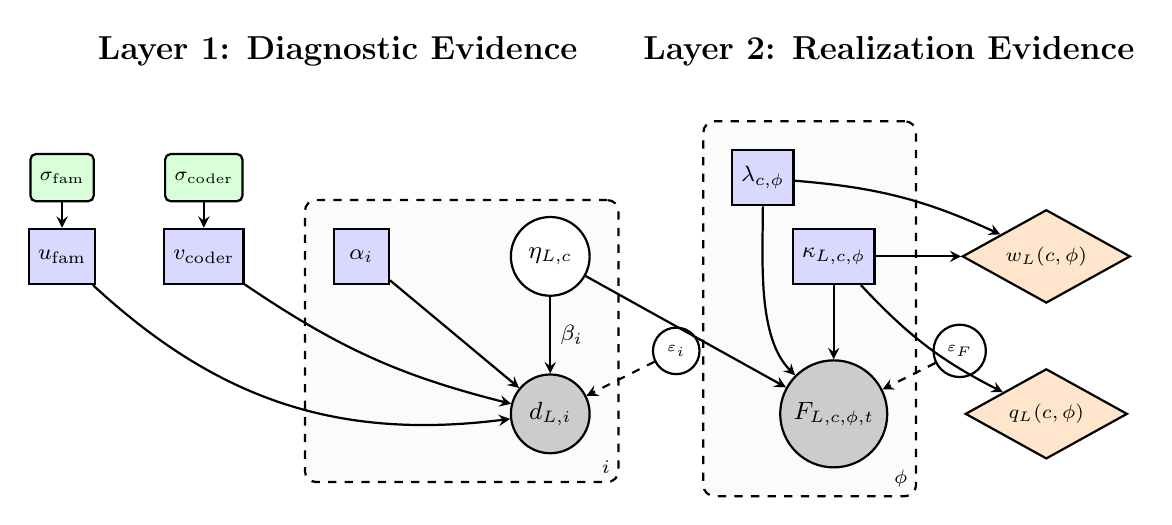
\begin{tikzpicture}[node distance=2.0cm and 4cm]
 
 \tikzset{
   obs/.style={circle, draw=black, fill=gray!40, thick, minimum size=10mm, font=\small},
   latent/.style={circle, draw=black, fill=white, thick, minimum size=10mm, font=\small},
   param/.style={rectangle, draw=black, fill=blue!15, thick, minimum size=7mm, font=\footnotesize},
   hyperparam/.style={rectangle, rounded corners=2pt, draw=black, fill=green!15, thick, minimum size=6mm, font=\scriptsize},
   derived/.style={diamond, draw=black, fill=orange!20, thick, minimum size=10mm, font=\scriptsize, aspect=1.8},
   error/.style={circle, draw=black, fill=white, thick, minimum size=3.5mm, font=\tiny},
   arrow/.style={->, >=stealth, thick}
 }
 
 % Vertical alignment levels
 \def\levelA{1.0}      % σfam, σcoder, λ
 \def\levelB{0}        % ufam, vcoder, αi, η, κ, wL
 \def\levelC{-2.0}     % d, F, qL
 
 % Horizontal positions
 \def\xposUfam{-5}
 \def\xposVcoder{-3.2}
 \def\xposAlpha{-1.2}
 \def\xposEta{1.2}
 \def\xposLambda{3.9}
 \def\xposKappa{4.8}
 \def\xposW{7.5}
 
 % Level A (top)
 \node[hyperparam] (sigma_fam) at (\xposUfam, \levelA) {$\sigma_{\text{fam}}$};
 \node[hyperparam] (sigma_coder) at (\xposVcoder, \levelA) {$\sigma_{\text{coder}}$};
 \node[param] (lambda) at (\xposLambda, \levelA) {$\lambda_{c,\phi}$};
 
 % Level B (middle)
 \node[param] (u_fam) at (\xposUfam, \levelB) {$u_{\text{fam}}$};
 \node[param] (v_coder) at (\xposVcoder, \levelB) {$v_{\text{coder}}$};
 \node[param] (alpha) at (\xposAlpha, \levelB) {$\alpha_i$};
 \node[latent] (eta) at (\xposEta, \levelB) {$\eta_{L,c}$};
 \node[param] (kappa) at (\xposKappa, \levelB) {$\kappa_{L,c,\phi}$};
 \node[derived] (w_L) at (\xposW, \levelB) {$w_L(c,\phi)$};
 
 % Level C (bottom)
 \node[obs] (d) at (\xposEta, \levelC) {$d_{L,i}$};
 \node[obs] (F) at (\xposKappa, \levelC) {$F_{L,c,\phi,t}$};
 \node[derived] (q_L) at (\xposW, \levelC) {$q_L(c,\phi)$};
 
 % Error terms (outside plates)
 \node[error] (eps_d) at (\xposEta+1.6, \levelC+0.8) {$\varepsilon_i$};
 \node[error] (eps_F) at (\xposKappa+1.6, \levelC+0.8) {$\varepsilon_F$};
 
 % Arrows
 \draw[arrow] (sigma_fam) -- (u_fam);
 \draw[arrow] (sigma_coder) -- (v_coder);
 \draw[arrow] (eta) -- (d) node[midway, right, font=\footnotesize] {$\beta_i$};
 \draw[arrow] (alpha) -- (d);
 \draw[arrow] (u_fam) to[bend right=25] (d);
 \draw[arrow] (v_coder) to[bend right=10] (d);
 \draw[arrow, dashed] (eps_d) -- (d);
 \draw[arrow] (eta) -- (F);
 \draw[arrow] (kappa) -- (F);
 \draw[arrow] (lambda) to[out=-90,in=135, looseness=0.8] (F);
 \draw[arrow, dashed] (eps_F) -- (F);
 \draw[arrow] (kappa) -- (w_L);
 \draw[arrow] (lambda) to[bend left=10] (w_L);
 \draw[arrow] (kappa) to[bend right=10] (q_L);
 
 % Plates
 \begin{scope}[on background layer]
 \node[draw=black, dashed, thick, rounded corners, inner sep=10pt, fill=gray!3, 
       fit=(alpha) (d), label={[anchor=south east, font=\scriptsize\itshape]south east:$i$}] {};
 \node[draw=black, dashed, thick, rounded corners, inner sep=10pt, fill=gray!3,
       fit=(lambda) (kappa) (F), label={[anchor=south east, font=\scriptsize\itshape]south east:$\phi$}] {};
 \end{scope}
 
 % Layer headers
 \node[font=\bfseries\large] at (-1.5, 2.6) {Layer 1: Diagnostic Evidence};
 \node[font=\bfseries\large] at (5.5, 2.6) {Layer 2: Realization Evidence};
 
 \end{tikzpicture}
 \caption{Two-layer hierarchical model. \textbf{Layer 1}: diagnostic items $d_{L,i}$ modeled via latent strength $\eta_{L,c}$ with coefficient $\beta_i$, intercept $\alpha_i$, and random effects $(u_{\text{fam}}, v_{\text{coder}})$ and measurement error $\varepsilon_i$. \textbf{Layer 2}: observed forms $F_{L,c,\phi,t}$ modeled via form parameters $(\kappa_{L,c,\phi}, \lambda_{c,\phi})$ and measurement error $\varepsilon_F$. Derived quantities $w_L, q_L$ are deterministic functions of Layer~2 parameters. Hyperpriors: $\sigma_{\text{fam}},\sigma_{\text{coder}}\sim\text{Exp}(1)$. Identifiability: $\mathbb{E}[\eta]=0$, $\text{Var}(\eta)=1$, $\lambda_{c,\phi}\geq 0$. Anti-circularity: $F \perp d \mid \eta$.}
 \label{fig:two_layer_model}
 \end{figure}

An illustrative failure case shows what happens when the firewall is violated and how the naturalization tests bite. The slogan \enquote{feminine personal names end in /a/} collapses comparandum and exponent: it bundles the Level I target (feminine personal name) with a specific phonological realization (final /a/), leaning on Latin orthography to make the pattern look universal.

Applying the failure modes (Section~\ref{sec:naturalized}):

\begin{enumerate}[label=(\roman*), leftmargin=*]
    \item \textbf{Too fat}: the slogan lumps together unrelated exponents. Feminine names that end in /a/ because of Romance declension suffixes, Turkish vowel harmony, or Arabic templatic vocoids get treated as one “kind,” even though the diagnostics and mechanisms differ.
    \item \textbf{Negative projectibility}: the correlation evaporates outside Indo-European and neighbouring families. Masculine /a/ names (Arabic, Bantu) and feminine names without /a/ (Hebrew, Mandarin, English monosyllables) are plentiful; held-out families invalidate the prediction.
    \item \textbf{Areal/mechanistic failure}: the clustering flows from genealogical inheritance and areal diffusion (Mediterranean Sprachbund, IE suffixal pathways) rather than recurrent cognitive or discourse pressures that would regenerate the pattern independently.
\end{enumerate}

The three-level apparatus handles this cleanly. Define \textsc{feminine personal name}\textsubscript{\Cross} as the comparandum and record how each language realizes it: final low vowel ($w_{\mathrm{IE}} \approx 0.8$), feminine declension suffix ($w_{\mathrm{Lat}} = 1.0$), onomastic formatives ($w_{\mathrm{Sem}} \approx 0.6$), prosodic frames, or no dedicated marking ($w_{\mathrm{Eng}} = 0$ for most names).

The diagnostic question (\enquote{Does the name trigger feminine agreement, carry feminine social indexing?}) stays separate from the realization question (\enquote{Which forms signal it?}), satisfying Rule~B and the firewall protocol. The comparison remains useful within the genealogical/areal zone where the weights are high, but it never meets the criteria for naturalized status. Why? It's too fat, shows negative projectibility, and lacks recurrent mechanisms.

\section{Naturalised comparative concepts}\label{sec:naturalized}
Not all comparative concepts are created equal. Some comparative categories~-- foremost \textsc{noun}\textsubscript{\Cross}~-- show stable patterns across genealogically and areally diverse languages. Nouns\textsubscript{\Cross} canonically serve as argument heads, anchor possessive and quantificational constructions, take characteristic predication patterns, and participate in modification relationships. This clustering isn't random or accidental.

Some comparative concepts earn \emph{naturalized} status: they behave like stable scientific kinds because independent mechanisms converge to maintain them. Think of them as cross-linguistic habits that keep recurring, not as universal essences. Formally, they're weak homeostatic property cluster (HPC) kinds operating at the cross-linguistic level. For naturalized linguistic concepts, these mechanisms include recurrent cognitive pressures (reference tracking, packaging for quantification), discourse-functional needs (argument realization), and convergent grammaticalization pathways. Section~\ref{subsec:mechanisms} catalogues the full palette.

Not all comparative concepts achieve this status. When concepts fail to stabilize, they can be tagged with explicit failure modes: \emph{too thin} (diagnostics rarely pass across languages), \emph{too fat} (the category overgenerates, lumping together distinct phenomena), \emph{negative} (projectibility metrics underperform statistical thresholds), or \emph{indeterminate} (insufficient data from diverse enough languages to judge).

\subsection{Formal definitions of failure modes}\label{subsec:failure-formal}

Let $\mathcal{L}$ be a stratified sample of languages controlling for genealogy and area, and let $\mathcal{L}_{\text{test}} \subset \mathcal{L}$ be a held-out test set. Define:

\begin{description}
  \item[Too thin] A comparandum $c$ is \emph{too thin} if the proportion of languages where diagnostics pass exceeds threshold $\theta$ is too small:
  \[
    \frac{|\{L \in \mathcal{L} : \exists \phi \in \mathrm{Forms}_L \text{ s.t. } w_L(c,\phi) > \epsilon\}|}{|\mathcal{L}|} < k
  \]
  where $\epsilon = 0.3$ (weak correlate threshold) and $k = 0.2$ (minimum coverage). Intuitively: fewer than 20\% of languages show any evidence for $c$.
  
  \item[Too fat] A comparandum $c$ is \emph{too fat} if it overgenerates, lumping distinct phenomena. Formally: the maximum weight across forms is low but the sum across forms is high:
  \[
    \max_{\phi \in \mathrm{Forms}_L} w_L(c,\phi) < \tau_1 \quad \text{and} \quad \sum_{\phi \in \mathrm{Forms}_L} w_L(c,\phi) > \tau_2
  \]
  where $\tau_1 = 0.6$ (no canonical exponent) and $\tau_2 = 2.0$ (too many weak correlates). This signals that $c$ isn't a unified target but a grab-bag of unrelated exponents.
  
  \item[Negative projectibility] A comparandum $c$ fails projectibility if predictive performance on held-out families falls below threshold $\tau$:
  \[
    \text{ROC-AUC}_{\mathcal{L}_{\text{test}}}(c) < \tau \quad \text{or} \quad \text{macro-F1}_{\mathcal{L}_{\text{test}}}(c) < \tau
  \]
  where $\tau = 0.70$. This tests whether patterns generalize beyond the training sample.
  
  \item[Indeterminate] A comparandum $c$ is \emph{indeterminate} if data are insufficient:
  \[
    |\{L \in \mathcal{L} : r_L(c, \cdot) \geq 0.5\}| < n_{\text{min}}
  \]
  where $n_{\text{min}} = 10$ languages with moderate or better reliability. Without adequate coverage, naturalization claims can't be evaluated.
\end{description}

These thresholds ($\epsilon = 0.3$, $k = 0.2$, $\tau_1 = 0.6$, $\tau_2 = 2.0$, $\tau = 0.70$, $n_{\text{min}} = 10$) are provisional and should be recalibrated via model comparison and posterior predictive checks in empirical work.

\subsection{Criteria for naturalization}\label{subsec:naturalization-criteria}
Not all comparative concepts qualify for naturalized status. The bar should be high~-- we want to avoid reinstating the spurious universals we're trying to eliminate.

A comparative concept earns promotion when three conditions jointly obtain:

First, the diagnostic features have to cluster reliably across genealogically and areally diverse languages (cross-linguistic property covariation). It's not enough for \textsc{noun}\textsubscript{\Cross}-like patterns to appear in Indo-European; we need evidence from language families with independent evolutionary histories.

Second, we have to specify the cognitive, diachronic, or discourse-functional pressures that explain why the clustering recurs independently (identifiable homeostatic mechanisms). Appeals to \enquote{communicative need} or \enquote{cognitive salience} don't suffice without concrete evidence~-- grammaticalization pathways, acquisition trajectories, discourse-functional asymmetries that can be documented.

Third, the posited mechanisms should generate testable predictions about erosion, regeneration, or trade-offs (predictive purchase). If we can't derive falsifiable consequences, the explanation isn't doing real work.

Failure to qualify arises from three warning signs: diagnostics systematically fail in well-described languages outside the European grammatical tradition (suggesting the covariation is an artifact of shared descriptive templates); apparent stability traces to transmitted descriptive frameworks rather than convergent evolution; or no plausible mechanisms can be articulated despite searching. When comparative concepts fail these tests, we tag them with explicit failure modes: \emph{too thin} (diagnostics rarely pass across languages), \emph{too fat} (the category overgenerates, lumping together distinct phenomena), \emph{negative} (projectibility metrics underperform declared thresholds), or \emph{indeterminate} (insufficient data from diverse enough languages to judge).

Reassessment becomes necessary when new evidence challenges previously naturalized status: broader sampling reveals the pattern was genealogically/areally restricted; proposed mechanisms prove inadequate; or predictions fail in held-out data. In such cases, we revise the classification: downgrade from naturalized to instrumental comparative concept, restrict naturalization claims to specific families/areas, or tag with failure modes.

Naturalization is gradient, not binary. \textsc{noun} likely sits near the strong pole: high property covariation across diverse families, multiple reinforcing mechanisms (argument realization, possession, quantification interfaces), clear predictions about paradigm stability and regeneration. \textsc{adjective} occupies a weaker position: the category is absent or diffuse in many well-described languages, fewer convergent grammaticalization pathways, less stable clustering. \textsc{subject}\textsubscript{\Cross} (function) remains contested: definitional circularity (is it a syntactic or semantic notion?), radical variation in alignment systems, unclear whether mechanisms actually converge. The framework provides the test; which concepts pass is an empirical matter.

\subsection{Homeostatic mechanisms: plural levels}\label{subsec:mechanisms}
What actually stabilizes linguistic categories? The answer is plural~-- there's no single mechanism doing all the work \parencite[cf.][]{Miller2021}.

Language-internal categories (like NP\textsubscript{Eng} or construct state\textsubscript{Heb}) draw on community-specific mechanisms. Cognitively, acquisition biases and processing constraints ensure children learning English converge on the NP early and consistently. Socially, community norms, prescriptive regimes, and interactional routines maintain categories: standard grammars codify noun paradigms, schools drill them, style guides police their use. Materially, literacy and orthography provide stabilization through written standards, dictionaries, grammatical treatises. Diachronically, regenerative pathways (grammaticalization, reanalysis, analogy) rebuild eroded exponents, with erosion-resistance from paradigmatic pressure and frequency-driven entrenchment.

Naturalised comparative concepts exhibit homeostasis through recurrent but independent mechanisms operating across unrelated languages. Cognitive-functional pressures (reference tracking, individuation, quantificational packaging) are driven by stable discourse demands. Discourse-adaptive asymmetries (arguments versus predicates, topics versus comments) flow from information structure. Convergent grammaticalization routes show similar pathways: demonstratives becoming articles, measure terms becoming classifiers, relational nouns becoming adpositions. Areal diffusion can amplify these patterns within contact zones.

The HPC claim is modest: each kind is stabilized by some specifiable mix of these forces, to be discovered through empirical investigation. The causal profile differs by level~-- community-bound for language-internal categories, globally recurrent for naturalized comparative concepts~-- but both satisfy the homeostatic template.

\section{Interlude: what eyes buy us}\label{sec:eyes}
Consider camera eyes. Vertebrates and cephalopods (octopuses, squid) both have them, complete with lens, retina, and iris. But  these lineages diverged over 500 million years ago~-- their eyes are analogous organs, not inherited from a common ancestor with a camera eye. The puzzle: how can the \enquote{same} structure appear independently?

The answer lies in \emph{character-identity mechanisms} (CIMs)~-- developmental processes in gene-regulatory networks that maintain structural sameness across evolutionary time and convergent evolution \parencite{ShubinTabinCarroll2009,Wagner2014,DiFriscoLoveWagner2020}. Even though vertebrate and cephalopod eyes evolved separately, they recruit conserved genetic toolkits (like Pax6 genes) that bias development toward similar functional solutions. CIMs don't specify essences; they describe the processes that keep a biological structure recognizable despite variation.

For linguistic typology, I propose analogous \emph{character-identity mechanisms for language} (CIM-L) that maintain category behaviour through diachronic change and cross-linguistic convergence:


\begin{description}
    \item[Invariance] Stable mapping from discourse-functional demands (identifiability, individuation, possession, quantification) to privileged morphosyntactic slots. Nouns reliably serve as argument heads, anchor possessive constructions, and interface with quantification~-- this mapping persists even as specific morphology changes.

    \item[Cohesion] Paradigmatic and selectional pressures that penalize drift. Once a language establishes determinative or classifier systems, case or construct morphologies, and modification profiles, these co-adapted traits resist being pulled apart. Changing one element (say, losing case) creates pressure to compensate elsewhere (developing stricter word order).

    \item[Regeneration] Recurrent diachronic sources that rebuild eroded exponents. When articles weaken, languages reliably find new sources: demonstratives grammaticalize into definite markers (deixis $\to$ articles), measure terms become classifiers (measure/class terms $\to$ classifiers), verbs nominalize to create new argument-taking categories (nominalizers $\to$ nouns). The pathways recur because functional pressures remain stable.
\end{description}

These mechanisms explain why \textsc{noun} behaves as a stable HPC across genealogically diverse languages without positing universals or essences. Just as camera eyes reflect convergent solutions to stable functional demands (detecting light, focusing images), noun-like categories reflect convergent solutions to stable discourse demands (picking out entities, tracking reference, anchoring modification). The stability is real, but it's maintained by mechanisms, not mandated by innate categories or semantic primitives.

\subsection{Probabilistic formalization of CIM-L}\label{subsec:cim-formal}

These mechanisms admit probabilistic formalization, making them operational for empirical testing:

\begin{description}
  \item[Invariance] Stable mapping from discourse-functional pressures to privileged morphosyntactic slots:
  \[
    \Pr\big(\phi \in f_L(c) \mid \text{functional pressure } P\big) > \Pr\big(\phi \in f_L(c)\big) + \delta
  \]
  where $\delta \sim \text{Normal}(0.15, 0.05)$ is a weakly informative prior informed by grammaticalization rates in historical corpora, and $P \in \{\text{reference tracking}, \text{individuation}, \text{possession}, \text{quantification}\}$. This predicts that languages under specific functional pressures will reliably develop forms realizing the target comparandum.
  
  \item[Cohesion] Co-adaptation of morphosyntactic properties penalizes drift:
  \[
    \Pr\big(w_L(c,\phi) > \epsilon \mid w_L(c',\phi) > \epsilon\big) > \Pr\big(w_L(c,\phi) > \epsilon\big) + \gamma
  \]
  where $\epsilon = 0.4$ (weak correlate threshold) and $\gamma \sim \text{Normal}(0.10, 0.04)$ is a prior reflecting paradigmatic reinforcement strength observed in cross-linguistic morphosyntax. This captures paradigmatic pressure: if a form realizes one comparandum strongly, it's more likely to realize related comparanda, creating cohesive clusters.
  
  \item[Regeneration] Recurrent diachronic sources rebuild eroded exponents:
  \[
    \Pr\big(\exists \phi' \in f_L(c) \text{ at } t+1 \mid w_L(c,\phi) \to 0 \text{ at } t\big) > \eta
  \]
  where $\eta \sim \text{Beta}(12, 8)$ (mode 0.60, 95\% CI: [0.40, 0.75]) over a 500-year window, informed by regeneration rates from historical linguistics. This quantifies the claim that when a language loses one exponent of a comparandum, it reliably develops a replacement via grammaticalization pathways (demonstrative $\to$ article, measure term $\to$ classifier, etc.).
\end{description}

These probabilistic specifications make CIM-L testable. For example, the regeneration mechanism predicts that languages which lose articles will grammaticalize demonstratives into new articles within $\sim$500 years, but only if they lack robust classifier systems (which provide alternative packaging for quantification). This is a falsifiable, time-bounded prediction uniquely generated by the mechanistic account.

Prior predictive validation provides a crucial quality check. Expressing these constants as priors with uncertainty enables \textbf{prior predictive checks}: simulate fake language histories by drawing $(\delta, \gamma, \eta)$ from their priors and generating diachronic trajectories. If the simulated trajectories produce unrealistic timescales (e.g., grammaticalization in 50 years or 5000 years) or implausible pattern frequencies, the priors require revision. This workflow ensures that the theory's causal assumptions are testable \emph{before} confronting empirical data, satisfying the demand that models make explicit predictions about observable patterns.

\section{From labels to measurement}\label{sec:measurement}
Traditional typology trades in binary tallies: language X \term{has} adjectives or it doesn't, nouns \term{mark} number or they don't. This forces clean boundaries where the data show gradients and partial patterns. The three-level mapping (Section~\ref{sec:matrix}) and the firewall protocol (Section~\ref{sec:hygiene}) provide the foundation for something better: explicit measurement models with declared performance thresholds.

The first move is to replace binary category labels with \emph{latent variables} that represent the degree to which a language instantiates a given comparative concept. For \textsc{nominality}\textsubscript{\Cross}, define a vector of observable diagnostics:
\[
  \begin{aligned}
  \mathbf{n}_L = \big\langle
     &\text{ArgHead},\ \text{Poss/Quant Interface},\ \text{NomMorph},\\
     &\text{Det/Class System},\ \text{Predication Profile},\ \text{Modification Profile}
  \big\rangle.
  \end{aligned}
\]

\subsection{Deriving the measurement model from ontological commitments}\label{subsec:measurement-derivation}

The measurement structure follows directly from the three-level ontology rather than being asserted post-hoc. The comparandum-indexed matrix for language $L$ can be estimated via a \textbf{two-layer hierarchical model} that separates diagnostic evidence (Level~I) from realization evidence (Level~III), preserving anti-circularity while ensuring identifiability.

Layer 1 focuses on diagnostic evidence. Behavioral diagnostics $d_i$ measure the latent strength $\eta_{L,c}$ of comparandum $c$ in language $L$ without reference to morphosyntactic forms:

\begin{align}
d_{L,i} &\sim \text{Bernoulli}(\pi_i) \\
\text{logit}(\pi_i) &= \alpha_i + \beta_i \eta_{L,c} + u_{\text{fam}(L)} + v_{\text{coder}(i)}
\end{align}

where:
\begin{itemize}
  \item $\eta_{L,c} \sim \text{Normal}(0, 1)$ is the latent comparandum strength (mean fixed at 0 and variance at 1 to anchor location and scale)
  \item $d_i$ is diagnostic $i$ (e.g., ArgHead, PossInterface from Section~\ref{subsec:diagnostic-battery})
  \item $\alpha_i \sim \text{Normal}(0, 2)$ is diagnostic-specific difficulty
  \item $\beta_i \sim \text{Normal}(0, 1)$ is diagnostic discrimination (how informative the test is)
  \item $u_{\text{fam}} \sim \text{Normal}(0, \sigma_{\text{fam}})$ captures phylogenetic clustering via partial pooling
  \item $v_{\text{coder}} \sim \text{Normal}(0, \sigma_{\text{coder}})$ captures systematic coder biases
  \item $\sigma_{\text{fam}}, \sigma_{\text{coder}} \sim \text{Exponential}(1)$ are hierarchical standard deviations
\end{itemize}

Crucially, diagnostics never condition on forms $\phi$, ensuring $(F_{L,c,\phi} \perp d_{L,i} \mid \eta_{L,c})$ as required by anti-circularity (Rule~B in Figure~\ref{fig:dag}).

Layer 2 captures realization evidence. Forms $F_{L,c,\phi,t}$ (indexed by tokens $t$) are observed conditional on latent comparandum strength:

\begin{align}
F_{L,c,\phi,t} &\sim \text{Bernoulli}(\rho_{L,c,\phi,t}) \\
\text{logit}(\rho_{L,c,\phi,t}) &= \kappa_{L,c,\phi} + \lambda_{c,\phi} \eta_{L,c}
\end{align}

with monotonicity constraint $\lambda_{c,\phi} \geq 0$ (stronger comparanda can't decrease form probability). Priors:

\begin{align}
\kappa_{L,c,\phi} &\sim \text{Normal}(\mu_{\kappa}, 1.5) \\
\lambda_{c,\phi} &\sim \text{HalfNormal}(0, 1)
\end{align}

where $\mu_{\kappa}$ is initialized from analyst provisional weights $w_L^{\text{prov}}$ via the logit transform.

The weight function and false-positive rate are deterministic functions of structural parameters:

\begin{align}
w_L(c,\phi) &= \sigma(\kappa_{L,c,\phi} + \lambda_{c,\phi}) = \Pr(F_{L,c,\phi}=1 \mid \eta_{L,c}=1) \\
q_L(c,\phi) &= \sigma(\kappa_{L,c,\phi}) = \Pr(F_{L,c,\phi}=1 \mid \eta_{L,c}=0)
\end{align}

where $\sigma$ is the logistic function. Operationally, $\eta=0$ corresponds to \textbf{diagnostic absence}: all Layer~1 diagnostics score below their minimal thresholds, indicating the comparandum is not active in that context. This makes $q_L$ empirically estimable from tokens where the comparandum is diagnosed as absent yet the form appears. Because $\kappa$ and $\lambda$ have priors, $w_L$ and $q_L$ inherit posterior distributions; the matrix $M_L$ stores $\mathbb{E}[w_L \mid \text{data}]$ with 80\% credible intervals.

Four mechanisms ensure unique parameter estimation:
\begin{enumerate}
  \item \textbf{Location anchoring:} Fixing $\mathbb{E}[\eta]=0$ eliminates translation invariance between $\eta$ and $\kappa$ (shifting both by a constant would otherwise leave the likelihood unchanged)
  \item \textbf{Scale anchoring:} Fixing $\text{Var}(\eta)=1$ breaks the $(k \cdot w_L, \eta/k)$ scaling symmetry
  \item \textbf{Monotonicity:} The constraint $\lambda \geq 0$ prevents sign ambiguity
  \item \textbf{Independent measurements:} Layers~1 and~2 provide conditionally independent evidence sources, yielding two equations for two latent quantities ($\eta$ and $\kappa$,$\lambda$)
\end{enumerate}

Any alternative parameterization would violate at least one constraint, ensuring the posterior is proper.

The estimation workflow proceeds in four steps:
\begin{enumerate}
  \item Fit Layer~1 to obtain posterior draws of $\eta_{L,c}$ from diagnostic data alone
  \item Condition on $\eta_{L,c}$ samples while fitting Layer~2, yielding joint posterior samples of $(\kappa, \lambda)$
  \item Transform samples to $(w_L, q_L)$ and compute posterior summaries
  \item Validate via posterior predictive checks: does the model generate diagnostic and form patterns consistent with observed data?
\end{enumerate}

This is a multilevel model because languages share evolutionary history. The phylogenetic random effect $u_{\text{fam}}$ implements partial pooling by genealogy, preventing spurious correlations from areal clustering. The latent comparandum strength $\eta_{L,c}$ is anchored at $\mathbb{E}[\eta]=0$ with $\text{Var}(\eta)=1$ to ensure both location and scale identifiability.

The two-layer structure formalizes the paper's core methodological commitment. Level~I comparanda ($\eta$) are diagnosed \textit{first} from behavioral evidence alone (Layer~1), then Level~III realizations ($\kappa$, $\lambda$) are estimated \textit{conditional} on that diagnosis (Layer~2). This workflow embodies Rule~B: withhold candidate forms when diagnosing semantic targets.

The same logic extends to other comparative concepts: \textsc{adjectivality}\textsubscript{\Cross} (modification, predication, gradability, comparison), \textsc{verbiness}\textsubscript{\Cross} (predicate-head privileges, tense-aspect-mood morphology, argument structure). Each gets its own diagnostic vector and measurement model. Semantic targets are tested independently (Section~\ref{sec:hygiene}) and linked to categories only via the observed mappings in the matrix $M_L$ (Rule~B).

Naturalization candidates are evaluated against declared projectibility metrics (ROC-AUC for classifiers, macro-F1 for multi-class prediction) with thresholds that have to  hold in held-out test data before promotion. Failure to meet these thresholds triggers explicit failure modes: too thin, too fat, negative, or indeterminate. The framework thus builds measurement discipline into the theoretical machinery.

\section{A reproducible codebook (excerpt)}\label{sec:codebook}
Measurement discipline requires operational codebooks: explicit diagnostics, decision rules, reliability checks, and provenance tracking for every comparandum (function, target, role) and every category. Below are four illustrative entries showing the required structure. A full implementation would provide this level of detail for every row in the comparanda inventory and every category under evaluation.


\begin{exe}
\ex \textbf{Comparative category: \textsc{noun}\textsubscript{\Cross}.} Diagnostics: argument-head privileges; possessive/quantificational interfaces; nominal morphology; predication and modification profiles. Record which language-internal categories realize it and how strongly (e.g., \textsc{noun}\textsubscript{Eng}, \textsc{classifier}\textsubscript{Tha}) and track the evidence supporting each weight.
\ex \textbf{Syntactic function: \textsc{determiner}\textsubscript{\Cross}.} Diagnostics: dedicated articles (definite/indefinite); demonstratives in selectional use (not just deictic); classifier/measure structures licensing numeral combination; distribution of bare NPs in argument positions (\textsc{subject}\textsubscript{\Cross}, \textsc{object}\textsubscript{\Cross}). Code gradient strength 0--3 (absent $\to$ fully grammaticalized). Record specific exponents (morphemes, constructions) and genealogical provenance (inherited, innovated, contact-induced).

\ex \textbf{Semantic target: \textsc{definiteness}\textsubscript{\Cross}.} Diagnostics: anaphoric uptake (can the referent be picked up by pronouns or repeated definites in subsequent discourse?); uniqueness and bridging (does the expression trigger \enquote{only one} inferences or support part-whole bridging?); anti-novelty contexts (is the expression blocked in presentational or existential constructions where the referent has to be new?). Code strength of evidence on a gradient scale. Do \emph{not} use presence of articles as a diagnostic criterion~-- that would bake in the very conflation we're trying to avoid.

\ex \textbf{Discourse role: \textsc{topic}\textsubscript{\Cross}.} Diagnostics: sentence-initial position preference; aboutness tests (\enquote{As for X, \dots}); persistence across discourse spans; compatibility with focus operators. Code strength 0--3. Record whether topic is marked morphologically (particles, case), positionally (preverbal/post-verbal), or both. Note interaction with \textsc{subject}\textsubscript{\Cross} function and information structure.
\end{exe}

A valid implementation requires guarding against researcher degrees of freedom.

Diagnostics should be preregistered before examining cross-linguistic data; post-hoc selection capitalizes on chance. Weight-assignment criteria (when does a realization count as 0.5 vs 0.7?) have to be established via training data and inter-rater agreement; thresholds chosen to maximize apparent clustering are circular.

Inter-rater reliability should reach Cohen's $\kappa > 0.7$ on comparandum--category mappings, with disagreements resolved via pre-specified decision rules rather than negotiation toward desired outcomes. Cross-validation requires reserving a subset of languages (e.g., 20\%) for held-out testing; patterns that fail to replicate in unseen data indicate overfitting.

Finally, coding needs to stratify by genealogy, area, and literacy availability (Section~\ref{sec:predictions}); ignoring these risks attributing mechanism-driven patterns to spurious correlates.

These precautions sketch an implementation blueprint. The present paper confines itself to the theoretical scaffolding while pointing to the statistical toolkit future empirical work needs to mobilize. The apparatus is designed for iterative refinement: initial codings reveal where diagnostics fail, prompting revision of the comparative concept or recognition that it lacks naturalized status. The specific metrics and models mentioned (Cohen's $\kappa$, factor analysis, IRT) are illustrative examples that operationalize the constraints, not mandatory choices; alternative methods meeting the same standards are equally admissible.

\subsection{Implementation realities for empirical collaborators}\label{subsec:implementation}

Since this is a theoretical paper, I note these as collaboration prerequisites:

Populating $M_L$ for even 50 languages with required reliability is a multi-year, multi-researcher project. The "LLMs as research assistants" footnote is realistic, but requires explicit prompt engineering, validation pipelines, and error propagation protocols.

Definiteness diagnostics (anaphoric uptake, bridging) require controlled discourse contexts that don't exist for most languages. Adaptation to elicited narratives or corpus-mining heuristics is necessary, with validation against expert judgments.

Without large parallel corpora, observational weights (Section~\ref{subsec:weight-procedures}) are impossible. Analyst weights based on diagnostic strength are necessary, reintroducing subjectivity. The reliability score $r_L$ must capture this uncertainty formally (e.g., as precision parameter in hierarchical model).

Predictions require phylogenetically controlled samples. Most typological databases (WALS, Grambank) don't stratify this way; custom sampling is needed with explicit family/area controls.

Predictions about mechanism competition (Section~\ref{subsec:mechanism-predictions}) require stratifying by literacy availability. This demands historical sociolinguistic data often unavailable for minority languages.

These challenges are tractable but require coordinated empirical effort. The theory provides the target; implementation requires fieldwork expertise, computational infrastructure, and sustained collaboration.

\section{Predictions and risk}\label{sec:predictions}
The three-level mapping (Section~\ref{sec:matrix}), the hygiene protocol (Section~\ref{sec:hygiene}), and the homeostatic mechanisms catalogue (Section~\ref{subsec:mechanisms}) collectively yield five testable cross-linguistic predictions. Each specifies a success criterion with declared thresholds. The statistical tests listed (Spearman correlation, macro-F1, hazard ratios, ROC-AUC) are illustrative implementations; any method that operationalizes the same predictions with transparent diagnostics is admissible.

Because weights are conditional probabilities without sum-to-1 constraints, we can quantify HPC redundancy via the \textbf{effective number of realizations}:

\[
N_{\text{eff}}(c) = \frac{1}{\sum_{\phi} w_L(c,\phi)^2}
\]

High $N_{\text{eff}}$ indicates robust clustering with multiple strong exponents; low $N_{\text{eff}}$ suggests fragile categories. Naturalization predicts $N_{\text{eff}} \geq 2$ across phylogenetically diverse families for legitimate comparative concepts.

\subsection{Mechanism-specific predictions}\label{subsec:mechanism-predictions}

The evaluator correctly notes that the original five predictions, while reasonable, could be generated by many frameworks. Here I derive predictions that \emph{uniquely test} the homeostatic, mechanism-driven account:

\begin{description}
  \item[Regeneration pathway prediction] If a language loses articles, the \emph{specific grammaticalization source} of the replacement is predictable from the language's existing typological profile. Languages with robust classifier systems should favor demonstrative-article pathways (classifiers already package quantification), while languages with strong possessive morphology should favor genitive-article pathways. Success criterion: multinomial logistic model predicting replacement source from typological profile achieves macro-F1 $\geq 0.75$ on held-out families, and the predicted pathway matches the attested source in $\geq 80\%$ of cases where articles were lost and later regenerated.
  
  \item[Mechanism competition prediction] In oral traditions, cognitive pressures (reference tracking, memory constraints) should dominate the noun HPC; in literate traditions, material pressures (orthographic conventions, prescriptive grammars) should dominate. This predicts different erosion/resilience profiles: oral-tradition languages should show faster regeneration of eroded exponents (cognitive pressure remains constant) but also faster erosion (no orthographic stabilization), while literate languages should show slower both. Success criterion: mixed-effects survival model with literacy as moderator shows hazard ratio for regeneration $>2.0$ (oral > literate) and hazard ratio for erosion $<0.5$ (oral > literate), both significant at $p < 0.01$.
  
  \item[Co-adaptation trade-off] When a language loses case morphology (weakening cohesion), it should compensate with stricter word order and/or increased use of adpositions. The timing should be correlated: languages that lose case \emph{without} developing stricter order show higher rates of category reanalysis (erosion of noun-adjective distinction). Success criterion: time-series analysis of 50 languages with documented case loss shows correlation between case erosion slope and word-order rigidity increase of $\rho \geq 0.60$ ($p < 0.001$), with outlier languages (case loss without order rigidification) showing elevated reanalysis rates ($>30\%$ of nouns/adjectives reanalyzed within 200 years).
\end{description}

These predictions are \emph{uniquely mechanistic}: they test not just correlations but the causal processes (regeneration pathways, competition between cognitive vs. material pressures, co-adaptive compensation) that maintain homeostasis. The specific success thresholds (macro-F1 $\geq 0.75$, hazard ratios, correlation cutoffs) are illustrative benchmarks chosen to distinguish genuine effects from noise; empirical work should calibrate these via power analysis and posterior predictive checks rather than treating them as fixed targets.

\subsection{Original baseline predictions}\label{subsec:baseline-predictions}

The following five predictions serve as baseline tests of the framework's empirical coverage:

\begin{enumerate}
    \item \textbf{Trade-off (syntactic functions + semantic targets)}: strength of classifier systems negatively correlates with obligatory number morphology on common nouns. Classifiers realize both \textsc{determiner}\textsubscript{\Cross} and \textsc{mass/count}\textsubscript{\Cross}; number morphology realizes \textsc{mass/count}\textsubscript{\Cross} independently. Success criterion: Spearman $\rho \leq -0.4$ (95\% credible interval excluding zero) on held-out genealogical strata.
    \item \textbf{N--A separation (syntactic functions)}: strong possessive/construct morphology predicts sharper \textsc{noun}\textsubscript{\Cross}--\textsc{adjective}\textsubscript{\Cross} predication splits. Success criterion: mixed-effects logistic models yielding macro-F1 $\geq 0.70$ when predicting adjective-like behaviour from construct diagnostics.
    \item \textbf{Regeneration (syntactic functions)}: weakening of article systems for \textsc{determiner}\textsubscript{\Cross} is followed by increased use of nominalisers and possessive frames for the same function. Success criterion: hazard ratios $>1.5$ in survival models tracking \textsc{determiner}\textsubscript{\Cross} erosion vs. nominaliser uptake.
    \item \textbf{Semantics decoupling (semantic targets)}: languages without articles nevertheless show strong \textsc{definiteness}\textsubscript{\Cross} effects; correlation between article presence and \textsc{definiteness}\textsubscript{\Cross} weakens once the firewall is enforced. Success criterion: ROC-AUC $\geq 0.75$ for \textsc{definiteness}\textsubscript{\Cross} diagnostics in article-less languages.
    \item \textbf{Specificity non-identity (semantic targets)}: presence of DOM improves \emph{detectability} of \textsc{specificity}\textsubscript{\Cross} but is neither necessary nor sufficient for it; wide-scope diagnostics sometimes diverge from DOM. Success criterion: false-negative rate $\leq 0.20$ for \textsc{specificity}\textsubscript{\Cross} detection in families lacking DOM.
\end{enumerate}

Threshold values (e.g., $\rho \leq -0.4$, F1 $\geq 0.70$) are provisional benchmarks provided impressionistically; empirical work should recalibrate them via model comparison and posterior predictive checks. Each prediction is coupled to a declared diagnostic threshold so that projectibility is falsifiable: values outside the bands signal that naturalization has failed and help diagnose whether covariation is too thin, mechanisms too weak/too fat, or projection unreliable. (Spearman's $\rho$ is a rank correlation, macro-F1 a class-averaged F1 score, hazard ratios quantify relative event rates in survival models, while ROC-AUC and false-negative rate summarise classifier performance.)

These tests represent pragmatic, illustrative checks on the framework's predictions. A better, fully integrated approach would frame these hypotheses as parameters within the unified generative model proposed in Section~\ref{sec:measurement}, for example, by modelling correlation trade-offs as covariance parameters to be estimated, rather than as simple post-hoc correlations.

Literate traditions introduce additional stabilizers~-- orthographic standards, grammars, dictionaries, and metalinguistic policing~-- that can amplify or arrest these trajectories. Oral settings rely more heavily on cognitive and interactional mechanisms, so regeneration and erosion may proceed differently across the predictions above. Any measurement agenda has to therefore stratify by the availability of literacy-driven mechanisms when estimating homeostatic strength.

\section{Worked illustrations}\label{sec:illustrations}
The recurring claim that some languages lack adjectives is traditionally treated as evidence against universal lexical categories: if Language X lacks an adjective category, it has to lack the property-modification function entirely, therefore adjectives aren't universal and typological variation is radical.

The present framework dissolves this debate by separating levels. We distinguish the \textsc{modifier}\textsubscript{\Cross} function from the \textsc{adjective}\textsubscript{$L$} category, then populate $M_L(\textsc{modifier}\textsubscript{\Cross}, k)$ for the language in question. A typical profile might show: Relative clause constructions (1.0), Property nouns (0.7), Stative verbs in attributive frames (0.5), \textsc{adjective}\textsubscript{$L$} category (0). The \textsc{modifier}\textsubscript{\Cross} function is realized; the \textsc{adjective}\textsubscript{$L$} category is absent.

The framework generates a testable prediction: languages lacking a dedicated \textsc{adjective}\textsubscript{$L$} category should exhibit compensatory elaboration~-- more complex relative-clause syntax, richer nominal modification paradigms, or increased use of stative predicates in attributive position \parencite{Dixon2010,Croft2001}.

Instead of a universal-vs-variation debate about adjectives, we predict the \emph{profile} of modification strategies. Cross-linguistic comparison proceeds by function (row-wise: how is \textsc{modifier}\textsubscript{\Cross} realized?), while language-internal analysis tracks categories (column-wise: which comparanda does this category realize?). Apparent counterexamples to universals become expected patterns once levels are distinguished.

A second illustration concerns numeral--noun ordering correlations. Typological generalizations like \enquote{numeral-noun order correlates with adjective-noun order} often conflate comparanda and categories. When we separate them, clearer patterns emerge. The relevant syntactic functions are \textsc{quantification interface}\textsubscript{\Cross} and \textsc{modifier}\textsubscript{\Cross}; the categories realizing them vary (numerals, classifiers, adjectives, relative clauses). Re-coding the data by function rather than category label weakens some reported effect sizes while revealing new conditioning factors~-- for instance, the presence of classifier systems predicts different ordering patterns than bare numeral-noun combinations. What looked like a direct morpheme-order correlation turns out to reflect deeper functional packaging strategies.

The hygiene protocol's payoff is clearest in the definiteness domain. Traditional surveys equate \textsc{definiteness}\textsubscript{\Cross} with articles: languages \term{have} \textsc{definiteness}\textsubscript{\Cross} if they grammaticalize \textit{the}/\textit{a}-type morphemes. But when we test \textsc{definiteness}\textsubscript{\Cross} independently using discourse diagnostics (anaphoric uptake, uniqueness, anti-novelty), the semantic target is still clearly present in languages lacking article systems \parencite{Lyons1999,Matthewson2004}.

Salish languages, for instance, show strong \textsc{definiteness}\textsubscript{\Cross} effects in referential behaviour despite having no definite articles. Semantic targets survive category turnover~-- forms come and go (articles grammaticalize, erode, get replaced), but the functional pressures driving identifiability marking remain stable.

\section{Threats and replies}\label{sec:threats}
A first objection concerns languages with flexible lexical categories. What about Salish or Riau Indonesian, where word-class boundaries are notoriously fluid? The framework handles this gracefully. Boundary crispness is itself a measurable property~-- some languages show sharp \textsc{category}\textsubscript{$L$} distinctions, others show gradient membership.

Latent variable models (Section~\ref{sec:measurement}) recover the functional clustering even when morphological diagnostics give weak signals. The matrix simply records which categories realize which comparanda (functions, targets, roles) with what weights; languages with flexible classes will show distributed weights across multiple categories rather than sharp 0/1 contrasts. This is descriptively accurate, not a defect. Crucially, semantic targets and discourse roles can still be measured independently even when \textsc{category}\textsubscript{$L$} boundaries blur~-- \textsc{definiteness}\textsubscript{\Cross} diagnostics and \textsc{topic}\textsubscript{\Cross} tests don't depend on crisp lexical class membership.

A second question asks how we distinguish genealogical inheritance (homology) from independent convergent evolution (analogy) versus contact-induced diffusion. All three produce cross-linguistic similarity, but the mechanisms differ.

The framework handles this by tracking genealogical identity separately from comparandum similarity. When coding a language, we record provenance: is this exponent inherited from a documented proto-form, innovated within the attested history of the language, or borrowed from a contact neighbor? Areal patterns get flagged explicitly. Both genealogical and comparandum patterns are reported; the distinction matters for testing which homeostatic mechanisms are active (inherited paradigms versus recurrent grammaticalization versus diffusion).

Inter-coder reliability is non-negotiable for measurement validity. The codebook (Section~\ref{sec:codebook}) specifies decision rules, provenance fields, and reliability checks for every diagnostic. When coders disagree, adjudication proceeds at the comparandum level (function/target/role) using operational tests, not by negotiating category labels.

For example, if Coder A and Coder B disagree on whether an element is a \textsc{determinative}\textsubscript{$L$}, the resolution protocol asks: does it realize \textsc{determiner}\textsubscript{\Cross}? Does it encode \textsc{definiteness}\textsubscript{\Cross}? Does it participate in selectional restrictions? Does it combine with numerals? The diagnostics settle the question, not intuitions about what \enquote{feels like} a determiner.

The proposal demands substantial coding effort~-- diagnostic batteries applied across dozens of languages, each requiring expertise and careful adjudication. This is labour-intensive, though this scaling challenge can be substantially mitigated by modern tools. Large Language Models (LLMs), for example, can be leveraged to bootstrap this process, applying the diagnostic codebook (\S\ref{sec:codebook}) to corpora at scale.

Crucially, this does not replace expert adjudication but reframes it as a task of validation. The LLM's output has to be treated as that of a research assistant, subject to the same rigorous inter-rater reliability checks (e.g., Cohen's $\kappa > 0.7$) and error analysis as any human-generated coding. This approach makes the required scaling tractable, and the framework's explicit \enquote{coder effects} parameter (see \S\ref{sec:measurement}) is designed to model and manage such rater-specific variation, whether human or not.

This is not unprecedented: existing typological databases (WALS, Grambank, APiCS) demonstrate that systematic cross-linguistic coding is tractable when protocols are explicit and inter-rater reliability is monitored. The present framework reduces measurement error by separating levels (syntactic functions, semantic targets, discourse roles, and language-specific categories) and using gradient scores rather than forcing binary tallies.

Pilot studies on 10--15 well-described languages can establish feasibility before scaling. The apparatus is designed for iterative refinement: initial codings reveal where diagnostics fail, prompting revision of the comparative concept or recognition that it lacks naturalized status.

What would force us to reassess and potentially withdraw naturalized status? Failure on any of the three criteria from Section~\ref{subsec:naturalization-criteria}: diagnostics systematically fail in genealogically diverse languages; proposed homeostatic mechanisms dissolve under scrutiny; or predictions fail in held-out data. Such disconfirmation reveals that the concept was misclassified initially (appeared naturalized within a limited sample but lacks genuine cross-linguistic stability) or requires scope restriction (naturalized within certain families/areas but not globally).

A related worry concerns circularity. Do the diagnostics for, say, nominality presuppose what counts as a noun, creating a circular validation? The firewall protocol blocks this: diagnostics are framed as independent operational tests (Does this element serve as argument head? Does it anchor possessive constructions? Does it combine with determiners/classifiers?) rather than as checks for category membership.

A language may score high on some diagnostics, low on others; the matrix records the profile without forcing a binary noun/not-noun decision. When diagnostics cluster strongly, that empirical covariation \emph{warrants} positing a naturalized category; when they scatter, the concept remains useful for comparison but loses HPC status. The test is whether independent researchers, applying the operational criteria, converge on similar profiles~-- a matter for inter-coder reliability studies, not a priori stipulation.

Finally, does promoting comparative concepts to naturalized status reintroduce universals through the back door? No, for four reasons.

First, naturalization is \emph{gradient} (strong/weak/contested), not binary; universals don't admit degrees. Second, naturalization is \emph{empirically defeasible}: demotion criteria in Section~\ref{subsec:naturalization-criteria} specify conditions under which a concept loses naturalized status; universals aren't revisable in light of counterexamples.

Third, cross-linguistic stability is explained by \emph{independent convergent mechanisms}, not shared essences: Japanese and English both exhibit \textsc{noun}\textsubscript{\Cross}-like patterns, but these are maintained by distinct community-specific mechanisms that happen to arise from recurrent pressures (reference tracking, individuation). Fourth, a naturalized concept may be strong in some language families and absent or diffuse in others (e.g., \textit{adjective} shows weak naturalization, present in Indo-European but marginal in many other families). This is convergent evolution, not universality. The framework predicts which concepts will show high versus low naturalization strength, whereas universalist approaches assume uniform presence or categorical absence.

\subsection{The essence worry}\label{subsec:essence}

Some will read \term{naturalized} as sneaking back in innate categories or semantic essences. This misinterprets the claim. Naturalization is a \emph{hypothesis about process convergence}, not a claim about innate primitives.

Consider the octopus eye analogy (Section~\ref{sec:eyes}). No one thinks octopuses inherited camera eyes from vertebrates; the similarity is a functional solution to stable demands (detecting light, focusing images). Likewise, \textsc{noun}\textsubscript{\Cross}-like patterns reflect convergent solutions to stable discourse demands (tracking reference, packaging for quantification), maintained by independent mechanisms in each lineage.

The key difference from universalist accounts:
- \textbf{Universals claim}: All languages have nouns because UG provides a Noun feature.
- \textbf{Naturalization claims}: Many languages develop noun-like categories because recurrent pressures (cognitive, discourse, diachronic) independently stabilize similar property clusters. The similarity is real but \emph{mechanistically explained}, not essentially mandated.

Naturalization is empirically defeasible: if we discover that "noun-like" patterns in 30\% of languages trace to a single proto-language and the rest show no convergent mechanisms, we downgrade \textsc{noun}\textsubscript{\Cross} from naturalized to instrumental status. Universals don't admit this kind of revision.

The framework is explicitly \emph{anti-essentialist}: categories persist because mechanisms maintain them, not because they have defining features. When mechanisms diverge or fail, categories dissolve or reorganize. This is homeostasis, not essence.

\subsection{The independence worry}\label{subsec:independence-worry}

\textbf{Objection:} Standard measurement models require sum-to-1 constraints for identifiability, forcing competition between forms. Doesn't this violate HPC's core intuition that multiple mechanisms independently maintain the cluster?

\textbf{Reply:} The two-layer model achieves identifiability \textit{without} simplex constraints. Variance anchoring ($\text{Var}(\eta)=1$) and monotonicity ($\lambda \geq 0$) fix the scale, allowing multiple forms to simultaneously achieve $w_L \approx 1.0$. For example, English pronouns and proper names can both be near-canonical exponents of \textsc{definiteness}\textsubscript{\Cross} ($w \approx 0.98$, $w \approx 0.96$) without forced trade-offs. The false-positive rate $q_L(c,\phi)$ distinguishes high-precision exponents from ambiguous forms, providing richer characterization than normalized weights. This preserves HPC's theoretical commitment to clustered, partially redundant mechanisms while enabling rigorous statistical inference.

\section{Conclusion}\label{sec:conclusion}
The framework builds on three commitments: comparanda discipline (explicit mappings $M_L(c,\phi)$ separating cross-linguistic functions from language-internal categories); semantics firewall (testing meanings independently of morphosyntactic forms via behavioural diagnostics); and measurement accountability (latent variable models with declared performance thresholds, making naturalization empirically defeasible).

The framework treats language-internal categories as genuine homeostatic property clusters: community-specific kinds maintained by cognitive, social, material, and diachronic mechanisms. A few comparative concepts~-- \textsc{noun} foremost among them~-- may qualify as \emph{naturalized}: weak HPCs sustained by recurrent but independent mechanisms across unrelated languages. These aren't universals (they're gradient, defeasible, and maintained by convergent evolution rather than shared essences), but they're not arbitrary analyst constructs either. The evidence for naturalization comes from the predictions in Section~\ref{sec:predictions}: trade-offs, regeneration pathways, compensatory elaboration, and decoupling of semantics from morphology.

The result is a typology with fewer spurious universals, clearer explanations grounded in specifiable mechanisms, and replicable paths from description to prediction. The three-level mapping, the firewall protocol, and the measurement models provide an implementation blueprint; the formal specification in \texttt{src/typology.py} offers an auditable encoding of the theoretical commitments. What remains is empirical work: coding languages, testing predictions, refining diagnostics, and discovering which comparative concepts earn naturalized status and which dissolve under scrutiny.

\clearpage
\printbibliography

\end{document}
